\chapter{Performance Evaluation}%
\label{eval}

This chapter, the performance of both of the networks outlined in
Chapter~\ref{implem} will be evaluated, such that their performance at playing
the game StarCraft II can be measured. The exact methodology for these tests is
described in Chapter~\ref{eval_method}.

Each section will be split into three, first evaluating the Deep Q network,
second the Convolutional network, and then finally comparing the two. The
results will mainly focus around the score achieved, which is the in-game is the
final score for the mini-game at hand, and for the Simple64 map this will
compare how the bot fairs across 5 games against various bots. For the
mini-games the overall comparison will allow comparisons with known baselines,
such that we can show how the agents stack up. For the Simple64 game where this
is not possible, it will instead focus on how the agent plays.

%TODO: I just made up the number here for how we will test the Simple64 map...
%so we should actually pick a number and make sure to update the above bit.

After this has been done for both the mini-games and the Simple64 map, the
results will compared overall to see what the advantages and disadvantages of
each network is, as well as comparing other parts of the networks such as
training time, and robustness.

Finally, before the conclusion, some of the additional parts of the trained
networks which are not directly linked to the performance of the network, but
do give insight into how the networks works will be shown. For example the
filters for the Convolutional network will be given here, as well as some
example outputs.

\section{Mini-games}

The mini-games are specific maps designed for training and testing different
skill requirements from the player. Each mini-game uses a different scoring
system, map and end goal. This makes it ideal for testing the agent on different
abilities for the agent to learn. Most of the mini-games incorporate some form
of randomness so that the agents do not learn to play using the same fixed
move-set. Because of this, the mini-games will be played 200 times with a
trained agent, and the mean and max scores will be recorded. This will allow a
suitable average to be taken, which takes into account the inherent randomness
of the mini-games.

For comparison, the results achieved by DeepMind are given in
Table~\ref{tab:deepmind}, as taken from the ``StarCraft II:\@ A New Challenge
for Reinforcement Learning'' paper.

\begin{table}[h]
    \centering
    \begin{tabular}{@{}c|c|rrrrrrr@{}}
        Agent & Metric &
        \rot{MoveToBeacon} & \rot{CollectMineralShards} &
        \rot{FindAndDefeatZerglings} & \rot{DefeatRoaches} &
        \rot{DefeatZerglingsAndBanelings} & \rot{CollectMineralsAndGas} &
        \rot{BuildMarines} \\ \midrule

        \multirow{2}{*}{Random Policy} & Mean & 1 & 17 & 4 & 1 & 23 & 12 & \textless{}1 \\
                                       & Max & 6 & 35 & 19 & 46 & 118 & 750 & 5 \\ \midrule

        \multirow{2}{*}{Random Search} & Mean & 25 & 32 & 21 & 51 & 55 & 2318 & 8 \\
                                       & Max & 29 & 57 & 33 & 241 & 159 & 3940 & 46 \\ \midrule

        \multirow{2}{*}{DeepMind Human Player} & Mean & 26 & 133 & 46 & 41 & 729 & 6880 & 138 \\
                                               & Max & 28 & 142 & 49 & 81 & 757 & 6952 & 142 \\ \midrule

        \multirow{2}{*}{StarCraft GrandMaster} & Mean & 28 & 177 & 61 & 215 & 727 & 7566 & 133 \\
                                               & Max & 28 & 179 & 61 & 363 & 848 & 7566 & 133 \\ \midrule \midrule

        \multirow{2}{*}{Atari-Net} & Best Mean & 25 & 96 & 49 & 101 & 81 & 3356 & \textless{}1 \\
                                   & Max & 33 & 131 & 59 & 351 & 352 & 3505 & 20 \\ \midrule

        \multirow{2}{*}{FullyConv} & Best Mean & 26 & 103 & 45 & 100 & 62 & 3978 & 3 \\
                                   & Max & 45 & 134 & 56 & 355 & 251 & 4130 & 42 \\ \midrule

        \multirow{2}{*}{FullyConv LSTM} & Best Mean & 26 & 104 & 44 & 98 & 96 & 3351 & 6 \\
                                        & Max & 35 & 137 & 57 & 373 & 444 & 3995 & 62
    \end{tabular}
    \caption{Scores achieved and outlined in the DeepMind ``StarCraft II:\@ A New
    Challenge for Reinforcement Learning'' paper.}%
    \label{tab:deepmind}%
\end{table}

\subsection{Deep Q Network}
%TODO: Evaluate all mini-games under DQN. As there is 8 I wouldn't go into
%detail for them all, mainly maybe 2 successes and 2 failures? The interesting
%ones basically. Give table of all results. Try not to do anything on curriculum
%learning etc.

Starting off with the Deep Q network, the mini-games that are to be used must
correlate with the network's state inputs. Since this network does not use an
image as the entire state input for the game, the mini-games chosen need to
relate the states that the network is designed to use. An example would be the
ability to move individual units. The Deep Q network does not yet support the
ability to move individual units since this is not in the networks available actions and
requires a much more complex actions to control individual units. This means
that the agent may perform sub-optimally in certain games.
On the other hand, due to the networks action space including actions that are
built up of multiple actions, this does also mean that in certain games the
agent has an advantage in that it can take a complicated action sequence.

Results are given in Table~\ref{tab:dqn_results}, where the mean and max score
achieved is given, as well as the number of episodes the agent was trained for
to achieve that score.

\begin{table}[h]
    \centering
    \begin{tabular}{@{}lrrr@{}}
        \toprule
        Map                         & Mean & Max & Episode Count \\ \midrule
        MoveToBeacon                & 5    & 21  & 2000          \\
        CollectMineralShards        & 11   & 23  & 2000          \\
        FindAndDefeatZerglings      &      &     &               \\
        DefeatRoaches               &      &     &               \\
        DefeatZerglingsAndBanelings &      &     &               \\
        CollectMineralsAndGas       & 2071 & 2814& 1000          \\
        BuildMarines                & 11   & 61  & 1000          \\ \bottomrule
    \end{tabular}
    \caption{Results for the Deep Q Network}%
    \label{tab:dqn_results}%
\end{table}

Looking at the table above, the Deep Q agent struggles with the action space
available. Due to the way the agent needs to test all combinations of state and
actions to identify the best action sequence, the agent is limited in the amount
of actions it is able to take and as so is unable to select specific units or
specific locations to send the units to. This meant that the agent struggles
with maps that require a complex action sequence of splitting units or moving
units to specific position.

The MoveToBeacon map is an example where the agent is unable to send the units
to the beacon, if the beacon is on the corners of the quads that the agent can
select. Q-Learning requires the agent to test different actions in a state to
identify the optimal action to take. If the action space is too large than the
agent will require a huge amount of training time such that the agent takes a
possible combination of actions to the goal.

However, it is possible to see the agent performs well on the
FindAndDefeatZerglings and BuildMarines map. Because the Deep Q actions are made
of multiple smaller action sets, the agent is able to execute the complex
commands with a single action. This makes it possible for the agent to take a
given action and evaluate the action without needing a large action space.

The agent is all the cases has learnt the correct sequence of actions to be taken for an optimal value approximation. The only limiting factor comes down the action space available to the agent. In the CollectMineralsAndGas mini-game, the agent has learnt to issue a command to the units to extract resources without calling any other actions that would use up these resources. The limiting factor is that the agent cannot create more CSV units, the units that farm and extract resources, due to the complexity of the action space.

\subsection{Convolutional Network}
%TODO: Evaluate all mini-games under CNN. As there is 8 I wouldn't go into
%detail for them all, mainly maybe 2 successes and 2 failures? The interesting
%ones basically. Give table of all results. Try not to do anything on curriculum
%learning etc.

In contrast to the Deep Q network, the Convolutional network does not have to
consider the state inputs, due to the only input being the screen and mini-map
data. This is both an advantage and disadvantage for the network, as it does not
need tuning potentially, but does also mean that the network lacks the required
information to perform well in some of the mini-games. For example, some
mini-games require the usage of resource management and knowing when to spend
resources to build units or buildings. Since the current number of resources is
not shown on the screen to the agent, it is unable to make decisions based on
this and as such suffers in these mini-games.
Similarly, there is no issues with action space due to having access to the
entire game action space. This means the agent is able to move multiple units
independently, and perform many actions. However, as there is no compound
actions, it is much harder for the network to perform complex actions, which
puts it at a disadvantage in later mini-games.

As before, Table~\ref{tab:cnn_results} contains the mean and max
scores achieved, as well as the number of episodes the agent trained for.

\begin{table}[h]
    \centering
    \begin{tabular}{@{}lrrr@{}}
        \toprule
        Map                         & Mean & Max & Episode Count \\ \midrule
        MoveToBeacon                & 26 & 32 & 2000 \\
        CollectMineralShards        & 84 & 110 & 3500 \\
        FindAndDefeatZerglings      &      &     &               \\
        DefeatRoaches               &      &     &               \\
        DefeatZerglingsAndBanelings &      &     &               \\
        CollectMineralsAndGas       & 1110 & 2025 & 2500 \\
        BuildMarines                & 2 & 8 & 2500 \\ \bottomrule
    \end{tabular}
    \caption{Results for the Convolutional Network}%
    \label{tab:cnn_results}%
\end{table}

The scores above highlight one of the known weakness of the network. Both of the
final two mini-games depend heavily on the current resources. Since this is
never passed to the network, the agent struggles heavily in these challenges.
That is because the agent never knows the state of the current resources, and as
such can not react to it. For a player, they can see they are able to build a
new gathering unit to increase their production, or to build a new building such
that they are able to store more resources, or a second command centre to build
units even faster. Since the agent never knows how many resources it has, it is
unable to formulate the concept of ``There is enough resources to build a new
unit/building'', so it struggles massively and the end result is worse than the
random policies DeepMind show. Similarly for BuildMarines, the agent never knows
to build marines or buildings to increase the unit cap and so on. This is why
the passing of additional variables is an important addition.

On the other side, the mini-games that depend solely on the screen input do very
well. The first mini-game is able to be completed to the level of an average
human player and the best DeepMind approaches. After this, the other mini-games
are predominantly close to the values given such that any changes can mostly be
put down to hyperparameter choices, since only a small sample of values was able
to be tested, due to time constraints.

\subsection{Network comparison}
%TODO: Compare/Contrast - Why did X network do well on some mini-game whilst the
%other did badly? Then spin it around and show why that helped it do well on a
%different one whilst the other struggled. I expect this will mainly compare the
%compound actions of the DQN vs the simple actions of the CNN.

The Deep Q network was able to learn the required actions to achieve the best results given the limitations in its action space. It would be favorable to make the agent learn the entire base sequence of the smaller action sets rather than giving an abstracted action such as build. In the implementation of the Q-Learning action space, the agent was designed to show an ability to learn using a deep neural network and not the complexity of its action space. To show the agents ability to learn, the actions needed to be simplified to a single command that would issue the sequence. For example, when the agent calls the attack action, a sequence of actions is executed. This includes selecting the the marine units by issuing a select point on the map, a select second point on map and then issuing the attack to the selected units. Such complex sequences, will require a lager network and more training episodes. 

\section{The Simple64 Map}
%TODO: Tiny bit on what, like 1 or 2 lines.

\subsection{Deep Q Network}
%TODO: Evaluate a number of games of the simple64 map under the DQN network.
%Give table of results, then a play by play of why it did good or bad across the
%games. Try not to do too much on the mini-games and then S64, since that is
%covered later.

\subsection{Convolutional Network}
%TODO: Evaluate a number of games of the simple64 map under the CNN network.
%Give table of results, then a play by play of why it did good or bad across the
%games. Try not to do too much on the mini-games and then S64, since that is
%covered later.

\subsection{Network comparison}
%TODO: Compare the networks again, explain why this time one did well and one
%did badly. Maybe talk about consistency here, how often they won, how their in
%game strategies compare etc.


\section{Transfer and Curriculum Learning}
%TODO: Add a few examples of the above, and show how it changes the results.
% I.e. show a bot going from MoveToBeacon -> CollectMinerals ->
% FindAndDefeatZerglings and compare that to learning with FindAndDefeatZerglings only.
% Similarly, compare learning a/many mini-games and then the Simple64 map as
% well as only the Simple64 map.
% Compare how well it does, time to learn, etc.

Training the Deep Q agent on the MoveToBeacon mini-game, the agent is required to point to the location of a beacon that will appear randomly on the map. The training was stopped and the agent was tested on the mini-game to show that the agent had learnt the correct actions to take. The same model was then tested on the CollectMineralShards mini-game without any training on the new map. The agent was able to collect the shards and perform well without the need to be retrained on the new mini-game. Scoring an average of 9, the agent performed almost as well as it would have been trained only on the CollectMineralShards map alone.

The Deep Q agent is then tested on its ability to attack on multiple mini-games. The agent is trained on the FindAndDefeatZerglings mini-game. This map required the agent to learn to search the map and kill the enemy units with little strategy required. The agent only needed to issue the attack command to increase the overall score. The agent is then tested on the DefeatRoaches and DefeatZerglingsAndBanelings. Again the agent was able to show the correct actions for the given state but with the limitation that the Deep Q agent is unable to control individual units. This is a necessary skill to achieving a higher score on these games as the agent needs to split the units and surround the enemies. The overall performance is similar to the agent being trained on each of the individual mini-games.


\section{Overall comparison}
%TODO: Overall comparison over both Accuracy and Generalisation and the networks as a
% whole, probably also including mention of training time.

\section{Network Information}
%TODO: Other additional parts of the network that hasn't been covered yet but
%wasn't applicable to the implem section. CNN - Filter displays etc. DQN - could
%we see how the QTable changes? etcetc

The figures below show the Deep Q score during training. We can see the score dip as the epsilon value is reduced due to the epsilon decay. The agent then learns the correct action to take in a given state.

\begin{figure}[h]
  \centering
  \begin{minipage}[b]{0.4\textwidth}
    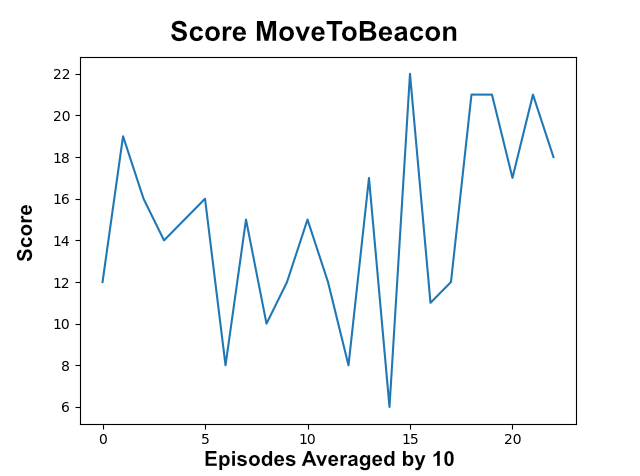
\includegraphics[width=\textwidth]{score_MoveToBeacon_train}
    \caption{Average of every 10 MoveToBeacon score during training}
  \end{minipage}
  \hfill
  \begin{minipage}[b]{0.4\textwidth}
    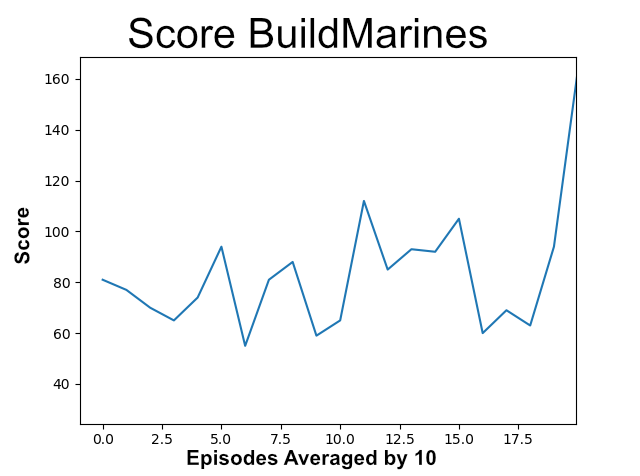
\includegraphics[width=\textwidth]{score_BuildMarines_train}
    \caption{Average of every 10 BuildMarines score during training}
  \end{minipage}
\end{figure}


\section{Conclusion}
%TODO: Broad conclusions of the networks based on the their performances.
